\documentclass{beamer}
\usepackage{csvsimple}

\title{Exploring Semantic Hierarchies to Improve Resolution Theorem Proving on Ontologies}
\subtitle{Stanley C. Small}


\setlength{\tabcolsep}{2pt}
\begin{document}
	\frame {
		\titlepage
	}
	
	\frame {
    	\frametitle{Agenda}
	Defense (2.5 Hours)
    	\begin{itemize}
		    \item Honors Thesis (1 Hour)
		    \begin{itemize}
     \item Presentation (20 min)
     \item Questions (40 min) 
   \end{itemize}
	        \item Honors Reading List (1 Hour)
	        		    \begin{itemize}
     \item Reading List Description (5 min)
     \item Reading List Discussion (55 min) 
   \end{itemize}
   \item Committee Deliberation (30 min)
    \begin{itemize}
     \item    Level of honors discussion
     \item Suggestions for Revision
   \end{itemize}
        \end{itemize}
	}
	
		    \frame{
	    \frametitle{Ontologies}
	    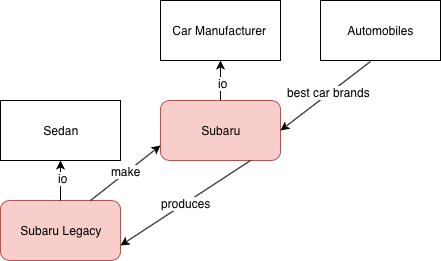
\includegraphics[width = \textwidth]{images/sample_ontology.png}
	}
	
				    \frame{
	    \frametitle{First Order Logic}
	    	
	    \[SubaruLegacy(myCar)\]
\[\forall x \; SubaruLegacy(x) \rightarrow Sedan(x)\]
\[\forall x \; Sedan(x) \rightarrow Automobile(x)\]
	}
	
			    \frame{
	    \frametitle{Theorem Proving}
	    
	    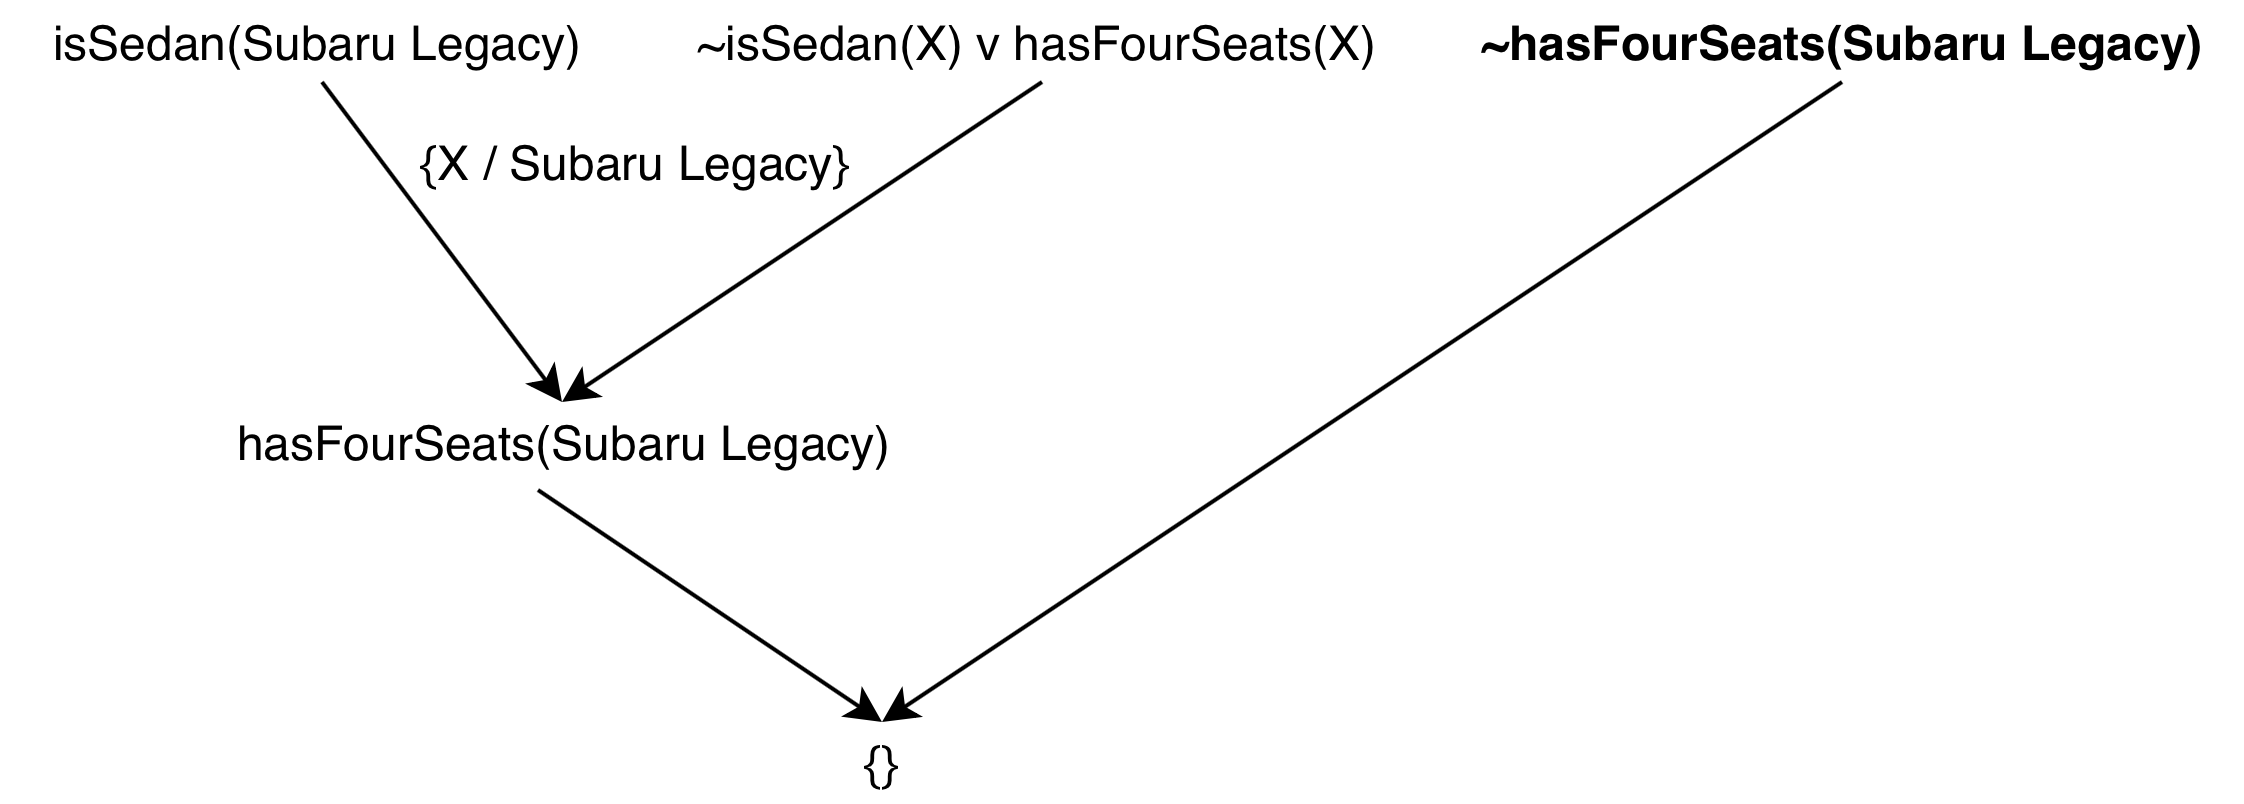
\includegraphics[width = \textwidth]{images/resolution_tree.png}
	}
	
	 \frame{
	    \frametitle{Semantic Hierarchies}
	    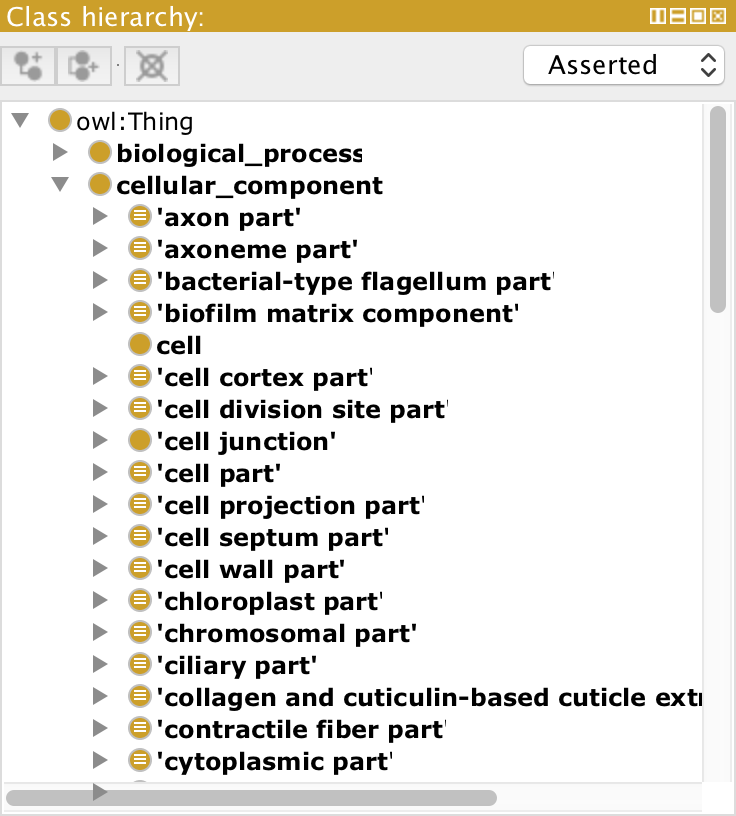
\includegraphics[width = 0.49\textwidth]{images/class-hierarchy.png}
	    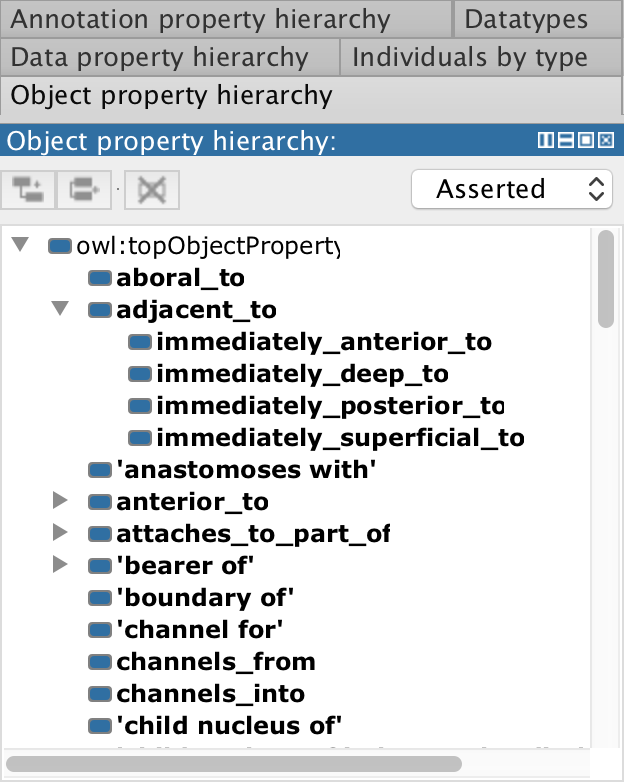
\includegraphics[width = 0.49\textwidth]{images/object-property-hierarchy.png}
	}
	
	    \frame{
	    \frametitle{Approach}
	    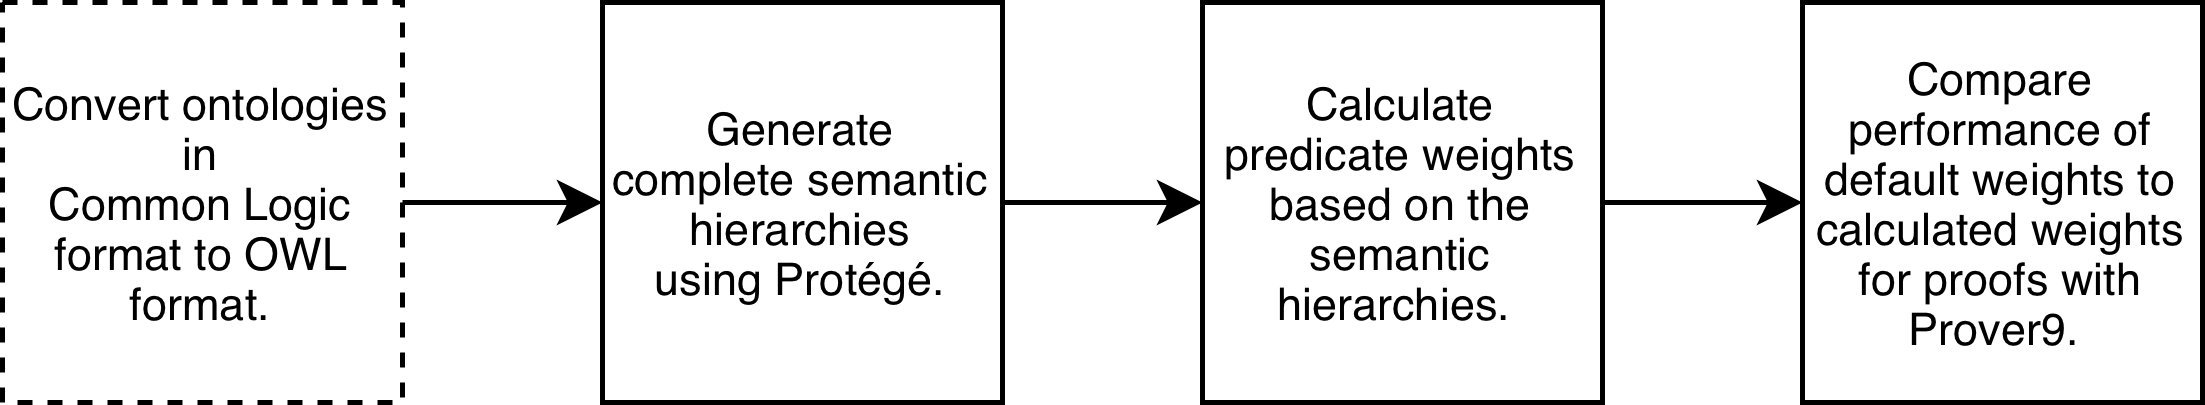
\includegraphics[width = \textwidth]{images/flowchart.png}
	}
	
	
			    \frame{
	    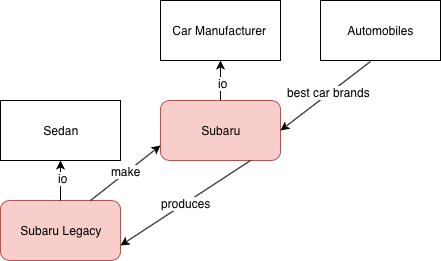
\includegraphics[width = \textwidth]{images/sample_ontology.png}
	}
	
	
	\frame{
	\frametitle{Function 1 Weights}
	\begin{itemize}
  \item weight(SubaruLegacy(x)) = 1. 
   \item weight(Sedan(x)) = 1. 
   \item weight(Automobile(x)) = 1. 
   \item weight(Minivan(x)) = 2. 
   \item weight(ToyotaSienna(x)) = 3. 
   \item weight(FordWindstar(x)) = 3. 
   \item weight(CarManufactuer(x)) = 10. 
  \item  weight(Produces(x,y)) - This is not defined as the conjecture contains no relationships. 
\end{itemize}
}

			    \frame{
	    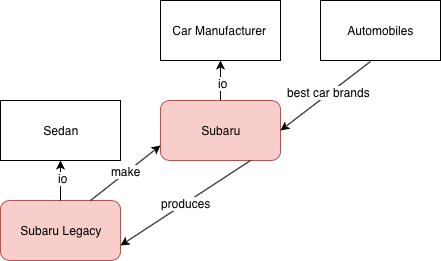
\includegraphics[width = \textwidth]{images/sample_ontology.png}
	}
	
	
	\frame{
	\frametitle{Function 2 Weights}
	\begin{itemize}
  \item weight(SubaruLegacy(x)) = 1. 
   \item weight(FordWindstar(x)) = 1. 
   \item weight(Automobile(x)) = 1. (LCA)
   \item weight(Sedan(x)) = 2. 
   \item weight(Minivan(x)) = 2. 
   \item weight(ToyotaSienna(x)) = 3. 
   \item weight(CarManufactuer(x)) = 3. 
  \end{itemize}
}

	

	 \frame{
	    	\begin{table}[h]
\centering
\csvautotabular{tests/multidim_space_voids/results.csv}
\caption{Results for the multidim\_space\_voids Ontology}
\end{table}
}
\frame {

\begin{table}[h]
\centering
\csvautotabular{tests/inch/results.csv}s
\caption{Results for the inch Ontology}
\end{table}
}
\frame{

\begin{table}[h]
\centering
\csvautotabular{tests/multidim_space_physcont/results.csv}
\caption{Results for the multidim\_space\_physcont Ontology}
\end{table}}
\frame{
\begin{table}[h]
\centering
\csvautotabular{tests/s.csv}
\caption{Overall Results}
\end{table}
	}
	
	\frame{
	    \frametitle{Limitations}
	    \begin{itemize}
	    \item Increase in clauses for inch ontology
	   \item \texttt{(all x all y (GED(x,y) \& GED(y,x) \& (all z (CH(z,x) -> CH(z,y))) -> CS(x,y))).} 
	   \item Semantic hierarchy has a depth of 2
	   \end{itemize}
	}
	
				    \frame{
	    \frametitle{Prover9 Output}
	    
	    \includegraphics[width = \textwidth]{images/inch_result.png}
	}
	
		\frame{
	    \frametitle{Summary}
	    \begin{itemize}
	    	\item When proving specific conjectures with few predicates on large ontologies, semantic hierarchies can focus the search of a resolution theorem prover. 
		\item Results of the experiments conducted indicate further work might yield lucrative results, especially for exceptionally large ontologies. 
		\item Tests demonstrated success in a relatively unexplored domain of research. 
	    \end{itemize}
	}
	
		    \frame{
	    \frametitle{Thank You}
	}
	
	
	    \frame{
	    \frametitle{Questions}
	}
	
		    \frame{
	    \frametitle{My Thoughts}
	    	\begin{itemize}
			\item A Mind for Numbers
			\item The Inner Game of Tennis
			\item Trying Not to Try
			\item I Ching
		\end{itemize}
	}
	  \frame{
		    \frametitle{My Career}
	    	\begin{itemize}
			\item Algorithms to Live By
			\item Black Mirror
			\item The Signal and the Noise
			\item Disrupted
		\end{itemize}
	}
	  \frame{
		    \frametitle{My Worldview}
	    	\begin{itemize}
			\item What Every BODY is Saying 
			\item Mr. Nobody
			\item The Lobster
			\item BoJack Horseman
		\end{itemize}
	}
	
\end{document}
